% ============================================================= %
%  --- Bell Database Article ---
% ============================================================= %

\documentclass[11pt, a4paper]{article}

% ------------------------------------------------------------- 
% Packages
% -------------------------------------------------------------
\usepackage{microtype} % Better typography
\usepackage{fontspec} % For loading fonts
\usepackage{fontawesome5} % For icons
\usepackage{parskip} % No paragraph indentation
\usepackage{ragged2e} % For better justification control
\usepackage{hyphenat} % For hyphenation control
\usepackage[left=2cm,right=2cm,top=2cm,bottom=2cm]{geometry} % Page margins
\usepackage{pgfplots} % For plots
\usepackage{pgf-pie} % For pie charts
\usepackage{amsmath} % For math
\usepackage{caption} % For captions


% -------------------------------------------------------------
% Font
% -------------------------------------------------------------
\usepackage{fontspec}
\setmainfont{Fira Code}


% -------------------------------------------------------------
% Styles
% -------------------------------------------------------------
\renewcommand{\abstractname}{} % Remove abstract title
\newlength{\abstractwidth}
\setlength{\abstractwidth}{0.8\textwidth}

% -------------------------------------------------------------
% Codeblocks
% -------------------------------------------------------------
\usepackage{listings} % For codeblocks
\usepackage{xcolor} % For colors
\definecolor{lgray}{gray}{0.9} % Light gray color

\lstdefinelanguage{CSS}{
  keywords={
    color, background, font, margin, padding, border, display, position,
    width, height, top, left, right, bottom, float, clear, overflow,
    text-align, vertical-align, line-height, letter-spacing, word-spacing,
    text-decoration, text-transform, font-family, font-size, font-weight,
    font-style, list-style, list-style-type, list-style-position,
    table-layout, border-collapse, border-spacing, caption-side, empty-cells,
    content, cursor, outline, visibility, z-index, zoom, filter, opacity,
    transition, animation, transform, box-shadow, text-shadow, border-radius,
    background-image, background-repeat, background-position, background-size,
    @media, @keyframes, !important
  },
  keywordstyle=\color{magenta},
  comment=[l]{//},
  morecomment=[s]{/*}{*/},
  commentstyle=\color{green},
  stringstyle=\color{purple},
  sensitive=true,
  morestring=[b]",
  morestring=[b]',
}

\lstdefinestyle{Pythonstyle}{
    language=Python,
    backgroundcolor=\color{lgray},
    commentstyle=\color{green},
    keywordstyle=\color{magenta},
    numberstyle=\tiny\color{gray},
    stringstyle=\color{purple},
    basicstyle=\ttfamily\footnotesize,
    breakatwhitespace=false,
    breaklines=true,
    captionpos=b,
    keepspaces=true,
    numbers=left,
    numbersep=5pt,
    showspaces=false,
    showstringspaces=false,
    showtabs=false,
    tabsize=2
}

\lstdefinestyle{CSSstyle}{
    language=CSS,
    backgroundcolor=\color{lgray},
    commentstyle=\color{green},
    keywordstyle=\color{magenta},
    numberstyle=\tiny\color{gray},
    stringstyle=\color{purple},
    basicstyle=\ttfamily\footnotesize,
    breakatwhitespace=false,
    breaklines=true,
    captionpos=b,
    keepspaces=true,
    numbers=left,
    numbersep=5pt,
    showspaces=false,
    showstringspaces=false,
    showtabs=false,
    tabsize=2
}

\lstdefinestyle{HTMLstyle}{
    language=HTML,
    backgroundcolor=\color{lgray},
    commentstyle=\color{green},
    keywordstyle=\color{magenta},
    numberstyle=\tiny\color{gray},
    stringstyle=\color{purple},
    basicstyle=\ttfamily\footnotesize,
    breakatwhitespace=false,
    breaklines=true,
    captionpos=b,
    keepspaces=true,
    numbers=left,
    numbersep=5pt,
    showspaces=false,
    showstringspaces=false,
    showtabs=false,
    tabsize=2
}


% ============================================================== %
%  --- Document Information ---
% ============================================================== %

\title{\Huge Structuring Bell Heritage: A Comprehensive Database Schema and Framework for Carillons and Bells}
\author{\LARGE{Jakob De Vreese} \\ \texttt{\small{jakobdevreese@gmail.com}}}
\date{March 2025}

% ============================================================== %
%  --- Document ---
% ============================================================== %

\begin{document}

% -------------------------------------------------------------
% Title Page
% -------------------------------------------------------------
\begin{titlepage}
    \newgeometry{top=6cm}
    \maketitle
    \thispagestyle{empty}
    \vspace{1cm}
    \begin{center}
        \small{last updated: \today}
    \end{center}
    \vspace{2cm}
    
    \begin{center}
        \rule{\textwidth}{0.4pt}
        \vspace{1em}
        
        \begin{minipage}{\abstractwidth}
            \setlength{\rightskip}{0pt plus 1fil} % Allow extra stretch on each line
            \justifying
            \noindent
            This research addresses a significant challenge in campanology: while enthusiasts and professionals 
            gather extensive data on bells and carillons, this valuable information often remains fragmented, 
            inconsistently structured, and inaccessible to the wider community. We propose the development of a 
            standardized framework for campanological data management — a comprehensive database schema designed 
            to accommodate the documentation needs for bells, carillons, and related heritage objects. This framework 
            aims to establish a foundation that balances standardization with flexibility, enabling individual 
            researchers and institutions to maintain autonomous databases while adhering to compatible structural 
            principles. The project consists of two key deliverables: first, a detailed entity-relationship model 
            that defines core data elements and their relationships; and second, an open-source Django web application 
            that implements this schema, providing accessible interfaces for data entry, management, and retrieval. 
            By establishing this standardized yet adaptable framework, we facilitate the potential integration of 
            distributed campanological datasets, thereby enhancing opportunities for comprehensive analysis, heritage 
            preservation, and collaborative research across both professional and amateur campanological communities.
          \end{minipage}
        
        \vspace{1em}
        \rule{\textwidth}{0.4pt}
    \end{center}

    \restoregeometry
\end{titlepage}

% -------------------------------------------------------------
% Table of Contents
% -------------------------------------------------------------

\clearpage
\setcounter{page}{1}
\pagenumbering{arabic}
\tableofcontents
\clearpage

% -------------------------------------------------------------
% Begin of the document
% -------------------------------------------------------------

\section{Introduction}

In the field of campanology, a wealth of valuable data is continuously gathered 
by both professional researchers and dedicated enthusiasts. This information 
encompasses a diverse range of attributes: physical dimensions of bells, acoustic 
properties, historical provenance, inscriptions, decorative elements, mechanical 
configurations, and the compositional arrangements of bell sets within carillons 
and towers. Despite this rich accumulation of knowledge, the campanological field 
faces a significant challenge: the lack of standardized methods for structuring, 
storing, and sharing this information in a consistent and accessible manner.

The current landscape of campanological data management is characterized by fragmentation 
and inconsistency. Individual researchers, institutions, and bell enthusiasts typically 
develop their own documentation methods, resulting in a patchwork of incompatible datasets. 
These range from handwritten notes and spreadsheets to custom-built databases with idiosyncratic 
schemas. While these approaches may serve immediate project needs, they create substantial 
barriers to knowledge sharing, comparative analysis, and comprehensive research across the broader field.

This fragmentation presents several critical limitations:

\begin{itemize}
    \item \textbf{Restricted Accessibility:} \\
        Valuable research remains siloed within individual projects or institutions, limiting potential insights from combined datasets.
    \item \textbf{Duplication of Effort:} \\
        Researchers frequently redocument the same bells due to lack of awareness or access to existing documentation.
    \item \textbf{Inconsistent Terminology:} \\
        The absence of standardized vocabulary and measurement protocols creates difficulties in comparing data between sources.
    \item \textbf{Limited Analytical Capacity:} \\
        The inability to easily aggregate distributed datasets hinders comprehensive statistical analysis and pattern recognition across larger samples.
\end{itemize}

This paper presents a solution to these challenges through the development of a comprehensive database schema and 
framework specifically designed for campanological research. Our approach balances the need for standardization 
with the flexibility required to accommodate the diverse documentation needs across the field. We propose both a 
conceptual data model — represented as an entity-relationship diagram — and its practical implementation as an 
open-source web application built using the Django framework.

The primary objectives of this project are to:
\begin{enumerate}
    \item Design and propose a flexibel, comprehensive and adaptable database schema for campanological data management.
    \item Develop an open-source, easy to use, web application that implements this schema.
    \item Facilitate the integration of distributed campanological datasets, enabling comprehensive analysis and collaborative research.
\end{enumerate}

\subsection{Itemize}

\begin{itemize}
    \item \textbf{Item 1:} \\
        Some information about item 1.
    \item \textbf{Item 2:} \\
        Some information about item 2.
    \item \textbf{Code: } \\
        This template has styles for \textbf{Python}, \textbf{CSS}, and \textbf{HTML}.
\end{itemize}
    
\section{Database Schema}

When designing a database schema for campanological data, we must consider the diverse range of attributes.
We start with the smallest unit we want to document: the bell. A bell has a set of physical properties, such absence
diamieter, height, weight and inscriptions, but also has a set of relationships with other entities, like bell founder. 
A bell hangs most of the time in a tower, wich gives away the geographical location, and can be part of a larger entity, the carillon. 
When we take this into account, we can start designing the database schema.

\begin{figure}[h!]
    \centering
    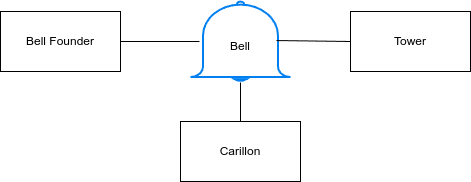
\includegraphics[width=0.8\textwidth]{images/basic_entities.png}
    \caption{Basic entities in the campanological database schema.}
    \label{fig:basic-entities}
\end{figure}

When we look at the basic entities in the campanological database schema, we see that the bell is the central entity.
When we put this central in our database, and we add the relationships between the entities, we get a readable and 
connectible database. To lay the basis for a standardization in this field, we off course need more. We want a minimum
of fields that every database in our field should have, and a standardized way of taking basic field measurements.

\subsection{Bell}

The bell is our starting point. The minimal attributes needed to describe a bell, in a way that it can't be confused with another bell, are:

\begin{itemize}
    \item \textbf{Founder:} \\
        The founder of a bell, this can be a person or a company. (Other enitie)
    \item \textbf{Weight:} \\
        The weight of the bell (in kilograms)
    \item \textbf{Pitch:} \\
        The pitch of the bell (in Hertz)
    \item \textbf{Diameter:} \\
        The diameter of the bell (in centimeters) - TODO - add more
    \item \textbf{Height:} \\
        The height of the bell (in centimeters) - TODO - add more
    \item \textbf{Inscriptions:} \\
        The inscriptions on the bell in words
    \item \textbf{Year:} \\
        The year the bell was cast.
    \item \textbf{Location:} \\
        The location of the bell. (Other entity) - TODO - add more

Other attributes can be added to the bell entity, but these are the minimal attributes needed to describe a bell. The researchers should strive 
to document these attributes as complete as possible for all bells.

\subsection{Founder}

The Founder entity presents unique modeling challenges in campanological documentation due to its inherent complexity. 
Bell founders may be individuals, family workshops, commercial enterprises, or combinations thereof, with varying historical 
naming conventions and organizational structures spanning centuries. Furthermore, founders often exhibit complex 
relationships — individuals may work under multiple establishments, companies may undergo name changes, and master founders 
may collaborate while maintaining distinct signatures.

To accommodate this complexity while ensuring standardization, we propose a structured approach to founder documentation with the following attributes:

\begin{itemize}
    \item \textbf{Primary Name:} The canonical name used for indexing and primary identification
    \item \textbf{Alternative Names:} Historical variants, orthographic differences, and aliases
    \item \textbf{Company Name:} May be blank or contain the name of a company or workshop.
    \item \textbf{Activity Period:} Documented years of bell-founding activity
    \item \textbf{Geographic Locations:} Principal locations of operation
\end{itemize}

This approach allows for precise documentation of complex cases: a bell signed by individual craftsmen working under a company name 
can be properly attributed to both entities while maintaining their relationship. Similarly, when a founder worked across multiple 
establishments during different periods, these associations can be preserved without sacrificing searchability. 
The schema enables researchers to query by either individual name or establishment, retrieving the complete attribution context 
regardless of entry point.

By implementing this structured yet flexible approach to founder documentation, we establish a foundation that accommodates 
historical complexity while facilitating standardized access and cross-referencing across distributed datasets.

\subsection{tower}

The tower entity is the geographical location where the bell is located. It is possible that a bell is not located in a tower, but
we still need to document the location of the bell. Then the tower entity can be filled in with minimal attributes and a remark that
the bell is not located in a tower. So in this case the tower name is a more generic class in our model, but since most bells are located 
in a tower, we can use the name for it to make the model more readable.

The items in the tower entity are:

\begin{itemize}
    \item \textbf{Name:} The name of the tower
    \item \textbf{Building:} The building attached to the tower, can be a church or can be empty when the tower in it self has a clear name.
    \item \textbf{geo_coordinates:} The geographical coordinates of the tower in longitude and latitude.
    \item \textbf{Adress:} The adress of the tower.
    \item \textbf{height:} The height of the tower.
    \item \textbf{height_bell:} The approxamte height of the bell in the tower.
    \item \textbf{remark:} A remark about the tower, can be used to document that the bell is not located in a tower or other remarks.
\end{itemize}

\subsection{Carillon}

The carillon entity is used to group bells in to a bigger entity, we know as a carillon. Since we sometimes have infomation on  a carillon but less on individual bells,
it should be possible to manually enter some calculated information on the carillon.
This also can be calculated automatically if all bells are entered in the database. 

The items in the carillon entity are:

\begin{itemize}
    \item \textbf{Established:} Year that the carillon was installed.
    \item \textbf{Number of bells:} The number of bells in the carillon.
    \item \textbf{Total weight:} The total weight of the carillon.
    \item \textbf{Transposition:} The pitch of the C bell in the carillon.
\end{itemize}

\subsection{Entity Relationship Diagram}

\section{Files}

We also want to enrich the database with files. This can be images, audiofragments, articles and more. 
The files should be possibel to be linked to anny individual entity like Tower, Bell, Carillon or Founder.

\section{Result}

\section{Web App}

\section{Conclusion}

During our research we have designed a comprehensive minimal database model, that could be 
the start of a more standardized apporach in documenting and sharing campanological information.
Our development of the open source web application is still ongoing and is hosted 
on GitHub. We welcome anny help on this subject. 

\end{document}